\section{Auswahl der Softwarekomponenten}
Im folgenden wird begründet, warum eine bestimmte Technologie ausgewählt wird und wie diese unser System ergänzt und warum diese optimal mit anderen Komponenten integriert werden kann.
\subsection{Auswahl eines geeigneten Extraktors}
Der Extraktor unseres Systems implementiert den ETL-Prozess und bringt diesen zur Ausführung. Seine Aufgabe ist das extrahieren der Daten, das transformieren der Daten in das Format des Zielsystems sowie das Laden der Daten in das Zielsystem. Implementiert wird dieser in der Programmiersprache Java. Grund hierfür ist, dass Java sehr weit verbreitet und etabliert ist sowie eine große Auswahl Frameworks und Bibliotheken bei der Entwicklung bietet. Zur Unterstützung in der Entwicklung wird ein Framework verwendet. Aus verschiedenen Gründe wird Quarkus eingesetzt. Ein großer Vorteil des Frameworks ist, dass es unter der Apache License 2.0 als Open Source Software eingesetzt werden kann. Außerdem bietet Quarkus eine sehr umfangreiche Auswahl an Erweiterungen für verschiedene Anwendungsfälle und unterstützt durch eine große Auswahl an Funktionen auch die Integration mit anderen Softwarekomponenten und Technologien. In der Praxis werden Anwendung in der Cloud häufig nach Rechenzeit und Speicherbedarf abgerechnet. Somit gewinnt die Optimierung der Anwendung auf Speicher- und Rechenzeitbedarf immer mehr an Wichtigkeit. Quarkus zeichnet sich durch eine schnelle Startzeit sowie die Optimierung für Container-Technologien und somit für Cloud-Umgebungen aus.\\
Ein weiterer Vorteil der Quarkus-Frameworks ist die Implementierung der Jakarta WS RS Schnittstelle, welche grundlegende Funktionalitäten für eine Unternehmensanwedung bietet. Die Implementierung einer offenen Spezifikation ermöglicht einen nahtlosen Umstieg auf ein alternatives Framework, welches ebenfalls diese Spezifikation implementiert, falls dieses notwendig ist. Alternative Frameworks wie z.B. Spring Boot implementiert z. T. proprietäre Spezifikationen und erschwert somit einen Wechsel, da häufig eine erneute Implementierung notwendig ist. Des weiteren bietet Quarkus Funktionen, um die Produktivität während des Entwickelns start zu verbessern. Eine Eigenschaft des Frameworks ist der Hot-Reload, welcher alle Änderungen des Codes automatisch in die laufende Entwicklungsinstanz einbringt und keinen Neustart der Anwendung erfordert. (vgl. Koleoso, 2020, S. 8)
\subsection{Auswahl eines geeigneten Datenbankmodells}
Der Mehrwert der Applikation für einen Anwender entsteht durch die Auswertung der Daten in unserem Zielsystem. Daher ist es besonders wichtig, auf ein Datenbankmodell zurückzugreifen, welches unseren Anwendungszweck, also das Integrieren mit einem Chatbot bestmöglich unterstützt. Im folgenden werden Datenbanken welche bei sehr spezifische Anwendungszwecken zum Einsatz kommen wie z.B eine Zeitstempel-Datenbank oder eine Key-Value-Datenbank nicht weiter betrachtet. Zur Auswahl stehen eine relationale Datenbank oder eine Graph-Datenbank. Um eine Entscheidung zu treffen, werden die beiden Datenbankmodelle anhand verschiedener Kriterien in Bezug zu unserem Anwendungsfall bewertet. Jedes Kriterium besitzt dabei eine Gewichtung. Ist das Kriterium besonders ausschlaggebend so ist die Gewichtung hoch. Eine ausführliche Erörterung der Kriterien folgt im Anschluss an die Tabelle.
\begin{table}[H]
\caption{Das Relationale und das Graph-Datenbankmodell im Vergleich}
    \begin{tabularx}{\textwidth}{|X|X|X|X|}
    \hline
    \textbf{Kriterium} & \textbf{Gewichtung} & \textbf{Relationale Datenbanken} & \textbf{Graph Datenbanken} \\ \hline
    Verknüpfungen         & 0,5         & 0 &  0 \\ \hline
    Skalierbarkeit         & 0,3         & Eintrag 6   & Eintrag 3        \\ \hline
    ACID-Eigenschaften         & 0,2         & 1,0    & 0,2      \\ \hline
    \textbf{Ergebnis}         &    0     & \textbf{1,0}    & \textbf{0,2}      \\ \hline
    \end{tabularx}
\end{table}
Verknüpfungen sind in unserem Anwendungsfall essenziell und werden somit stark gewichtet. Relationale Dantenbanken verbinden Entitäten durch logische Verknüpfungen. Während dieses Vorgehen für eine gute Lesbarkeit für menschliche Anwender bietet, wird dadurch die Zeit einer Anfrage beeinträchtigt. Folgende Grafik vergleicht die Abfragezeiten vom Finden von Entitäten, welche durch eine bestimmte Tiefe (Anzahl der Verknüpfungen) von der Ausgangsentität entfernt sind.

\begin{figure}[H]
\centering
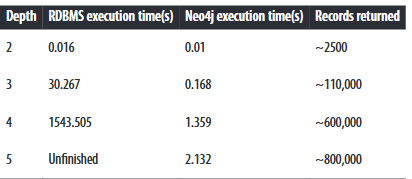
\includegraphics[scale=.6]{dateien/table.png}
\captionsetup{font=small, labelfont=bf, justification=centering}
\caption{Vergleich der Abfragezeit von Entitäten in RDBMS und Graph Datenbanken (vgl. Robinson, Webber und Eifrem, 2025, S. 21)}
\label{fig:meine-grafik}
\end{figure}
Graph Datenbanken implementieren die Verknüpfungen von Entitäten durch physische Pointer. Es wird eine Relationale Datenbank mit einer Graph Datenbank verglichen (Neo4J). Hierbei wird direkt der Speicherort referenziert. Für unseren Einsatzzweck benötigen wir eine Datenbank, welche stark auf die Verknüpfung von Daten optimiert ist und bewerten somit die Graph Datenbank höher.\\
Graph Datenbanken erreichen eine höhere Skalierbarkeit im Vergleich zu relationalen Datenbanken. Dies wird in Abbildung 2 ebenfalls sichtbar. Es zeigt sich ein sehr starker Anstieg der Ausführungszeit bei Relationalen Datenbankmanagementsystemen und ein weniger starker Anstieg bei Graph Datenbankmanagementsystemen. Dies deutet darauf hin, dass Graphdatenbanken effizienter mit großen Datenmengen umgehen können.
\subsection{Chancen und Eigenschaften von Graphdatenbanken}
Graphdatenbanken bestehen aus Knoten und Kanten. Knoten werden mittels Kanten miteinander verbunden und ermöglichen somit ein traversieren der Datenstruktur. Des Weiteren besteht die Möglichkeit den Kanten mit Werten zu versehen, welche als Gewichtung oder Distanz dienen können und somit die Verknpüfung zwischen zwei Knoten quanitifizieren und genauer beschreiben. Graphen, welche Kanten beinhalten, die mehr als 2 Knoten miteinander verknüpfen werden Hypergraphen genannt. Kanten die mehr als 2 Knoten verknüpfen werden Hyperkanten genannt [ZITAT Limitations of graph Databases]. \\Auch wenn eine Graphdatenbank andere Eigenschaften als eine Relationale Datenbank aufweist, finden sich dennoch Elemente aus einer Relationalen Datenbank wieder. Beispielsweise werden Knoten und Kanten als Tabellen gespeichert. Alle Knoten eines Types können mitsamt dessen Attribute wie bei einer relationalen Datenbank per Abfrage ausgegeben werden.\\
Durch den Einsatz von Kanten können Knoten sehr einfach miteinander verknüpft werden. Im Gegensatz zu Relationalen Datenbanken sind somit keine Joins mehr notwendig, da Knoten auf ebene der Datenhaltung direkt miteinander verknüpft werden. Dadurch werden Strukturen geschaffen, welche von einer Künstlichen Intelligenz relativ einfach verknüpft und zu einem Sachverhalt zusammengeführt werden können.
Graphdatenbanken können extrem schnell durchsucht werden und es können Muster im Aufbau des Graphen entdeckt werden.\\
% Leistung und Skalierbarkeit von Graphdatenbanken
Graphdatenbanken sind gut geeignet für große Datenmengen. Graphdatenbanken, die im Bereich Big Data eingesetzt werden, werden als \glqq Big Graphs\grqq\: bezeichnet und können bis zu 1 Milliarde Knoten enthalten, welche durch bis zu 140 Milliarden Kanten miteinander verknüpft sind.\\
% Wo werden diese Datenbanken eingesetzt
Graph Datenbanken decken ein großes Einsatzgebiet ab und werden meist dann eingesetzt, wenn die zu Grunde liegenden Daten stark verknüpft sind. Dies ist u. A. bei sozialen Netzwerken, Wissensgraphen und bei sogenannten Recommendation Engines, also Systeme, welche Vorschläge basierend auf existierenden Daten liefern, der Fall. So können Graphdatenbanken sehr gut mit Verknüpfungen umgehen. Ein weiterer Anwendungsfall für welchen sich Graphdatenbanken gut eignen sind im Umgang mit Daten, welche nur eine schwache Struktur aufweisen. [ZITAT Limits of Graph Databases] \\
Die Entwicklung und Leistung der aktuell verfügbaren Graphdatenbanken gilt als ein entscheidender Faktor für die Entwicklung von leistungsstarken Künstlichen Intelligenzen. (vgl. Fensel et al. 2020, S. 96)
\subsection{Überblick über die Jira Cloud}
Dieses Kapitel gibt einen Überblick über die wichtigsten Aspekte und Elemente in Jira und wozu diese verwendet werden. Die Jira Software ermöglicht das Verwalten von Arbeitsvorgängen, welche als Tickets im System angelegt werden können. Jira-Tickets können in verschiedenen Arbeitsbereichen wie z.B dem Projektmanagement oder der Softwareentwicklung eingesetzt werden, um Aufgaben zu planen. Die Jira Software steht als hybrides Modell zur Verfügung und kann demnach als Data-Center Version selbstständig betrieben oder als Cloud Produkt gebucht werden. Die Inhalte dieser Arbeit basieren auf der Cloud Version der Jira Software. Das System unterstützt primär die Durchführung von Projekten durch den Einsatz von agilen Vorgehensmodellen. Standardmäßig bietet das System u. A. die agilen Methoden Scrum und Kanban an. In einer Jira Cloud Instanz können mehrere Projekte erstellt werden. Diese Projekte enthalten verschiedene Vorgänge, welche inhaltlich ähnlich sind. Die Vorgänge können verschiedene Zwecke erfüllen, welche immer durch den jeweiligen Vorgangstyp des Tickets verdeutlicht werden. Neben der Möglichkeit, Vorgangstypen selbst zu erstellen gibt es bereits einige Vorgangstypen, welche standardmäßig im System vorhanden sind. Zu den bereits vorhandenen und gängigen Vorgangstypen zählt der \glqq Bug\grqq\:, welcher verdeutlicht, dass es sich bei dem Vorgang um ein Problem handelt, welches gelöst werden soll. Auch die \glqq Story\grqq\: ist bereits im Jira System vorhanden und stellt einen Arbeitsvorgang da, welcher die Implementierung eines neuen Features beschreibt. Ein Ticket kann in weitere Aufgaben unterteilt werden. Diese werden als Unteraufgaben bezeichnet. Ein Ticket oder eine Unteraufgabe kann einen Ersteller haben und einem Bearbeiter zugewiesen sein.\\
In Jira besitzt ein Ticket immer einen Workflow. Ein Workflow ist eine Verknüpfung von verschiedenen Status zu einem Arbeitsablauf. Ein Workflow besitzt immer einen Anfrangsstatus sowie einen oder mehrere Endstatus. Wird ein Vorgang neu erstellt befindet sich dieser im Anfangsstatus des ihm zugeordneten Workflows. Der Status eines Tickets gibt immer Aufschluss über dessen den Bearbeitungsstand. So kann ein Status beispielsweise andeuten, dass ein Ticket beispielsweise noch offen, sich in Bearbeitung befindet oder die Bearbeitung abgeschlossen ist.